\documentclass{article}

\usepackage{Sweave}
\begin{document}
\Sconcordance{concordance:UEbung2.tex:UEbung2.Rnw:%
1 2 1 1 0 8 1 1 4 3 0 3 1 7 0 1 1 8 0 1 2 2 1 1 2 1 0 1 3 2 0 3 1 4 0 2 %
2 1 0 1 1 6 0 1 1 5 0 5 1 4 0 1 2 3 1 1 4 3 0 1 3 2 0 1 2 4 1 1 9 6 0 1 %
2 2 1 5 0 1 3 2 1 1 2 1 0 1 3 2 0 1 2 2 1 1 6 4 0 2 2 2 1 4 0 1 2 3 1 1 %
3 2 0 2 1 3 0 2 2 8 0 1 1 8 0 1 2 2 1 1 2 1 0 1 1 4 0 2 2 1 0 1 1 6 0 1 %
2 4 1 4 0 1 2 4 1 1 2 1 0 2 1 1 2 2 1 1 2 2 1 2 2 2 1 9 0 1 2 1 3 1 2 4 %
1 1 2 1 0 2 1 1 2 2 1 1 2 2 1 2 2 2 1 9 0 1 2 1 3 1 2 3 1 1 4 3 0 1 4 2 %
0 1 2 3 1 1 8 6 0 1 1 12 0 1 2 4 1 1 2 7 0 1 2 2 1 1 2 7 0 1 2 2 1 1 2 %
7 0 1 2 2 1}




\section{Übung 2}
\subsection{Aufgabe 9}
\subsubsection{a}

\begin{Schunk}
\begin{Sinput}
> income <- c(2, 4, 6, 4, 7, 5, 7, 4, 3, 5,
+             5, 8, 6, 3, 5, 2, 9, 4, 5, 6, 
+             8, 3, 10, 5, 4, 3, 7, 4, 6, 4)
> income.table <- table(income)
> income.proptable <- prop.table(table(income))
> addmargins(income.table)
\end{Sinput}
\begin{Soutput}
income
  2   3   4   5   6   7   8   9  10 Sum 
  2   4   7   6   4   3   2   1   1  30 
\end{Soutput}
\begin{Sinput}
> round(income.proptable * 100, 2)
\end{Sinput}
\begin{Soutput}
income
    2     3     4     5     6     7     8     9    10 
 6.67 13.33 23.33 20.00 13.33 10.00  6.67  3.33  3.33 
\end{Soutput}
\end{Schunk}

\subsubsection{b}

\begin{Schunk}
\begin{Sinput}
> library("graphics")
> income <- c(2, 4, 6, 4, 7, 5, 7, 4, 3, 5,
+             5, 8, 6, 3, 5, 2, 9, 4, 5, 6, 
+             8, 3, 10, 5, 4, 3, 7, 4, 6, 4)
> income.table <- table(income)
> income.proptable <- prop.table(table(income))
> barplot(income.table)
\end{Sinput}
\end{Schunk}
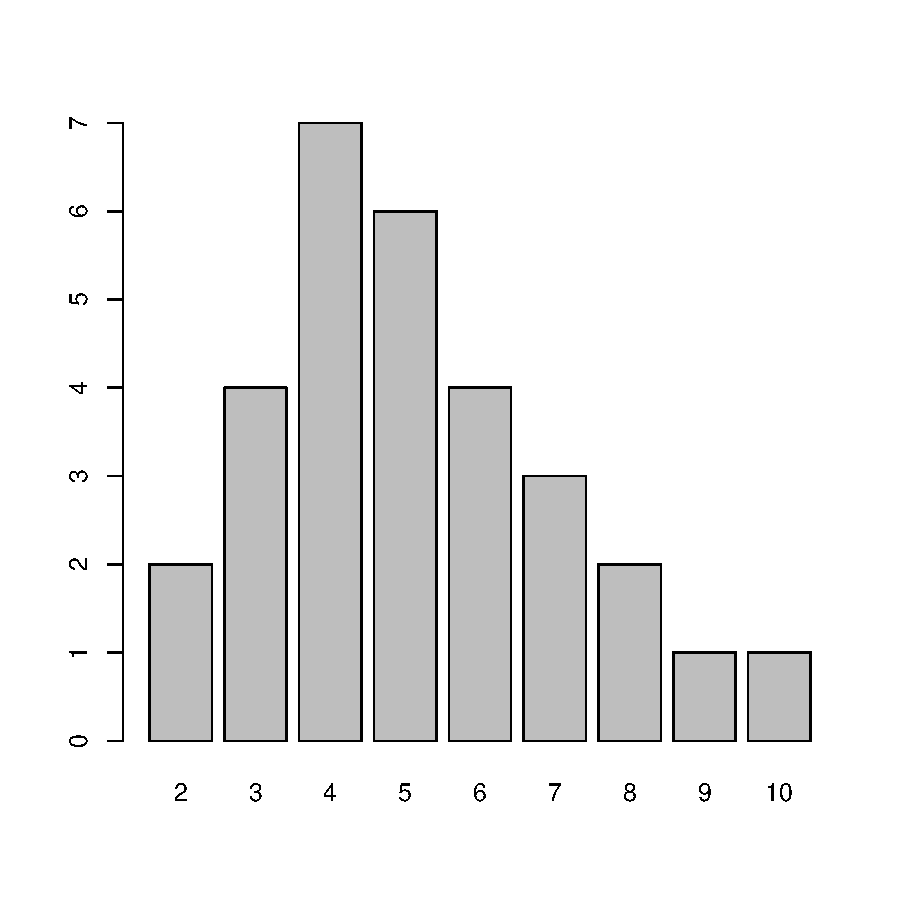
\includegraphics{UEbung2-002}

\begin{Schunk}
\begin{Sinput}
> income.cumulatedSum <- cumsum(income.table)
> income.cumulatedSum
\end{Sinput}
\begin{Soutput}
 2  3  4  5  6  7  8  9 10 
 2  6 13 19 23 26 28 29 30 
\end{Soutput}
\begin{Sinput}
> names(income.cumulatedSum)
\end{Sinput}
\begin{Soutput}
[1] "2"  "3"  "4"  "5"  "6"  "7"  "8"  "9"  "10"
\end{Soutput}
\begin{Sinput}
> plot(income.cumulatedSum, type = "l", axes=FALSE, col="blue", ylab = "Kumulierte Häufigkeit", xlab = "Umsatz")
> axis(1, at=1:length(names(income.cumulatedSum)), labels=names(income.cumulatedSum))
> axis(2, at=1:tail(income.cumulatedSum, n=1), labels=1:tail(income.cumulatedSum, n=1))
> abline(v=1:length(names(income.cumulatedSum)), col="lightgray")
> abline(h=1:max(income.cumulatedSum), col="lightgray")
\end{Sinput}
\end{Schunk}
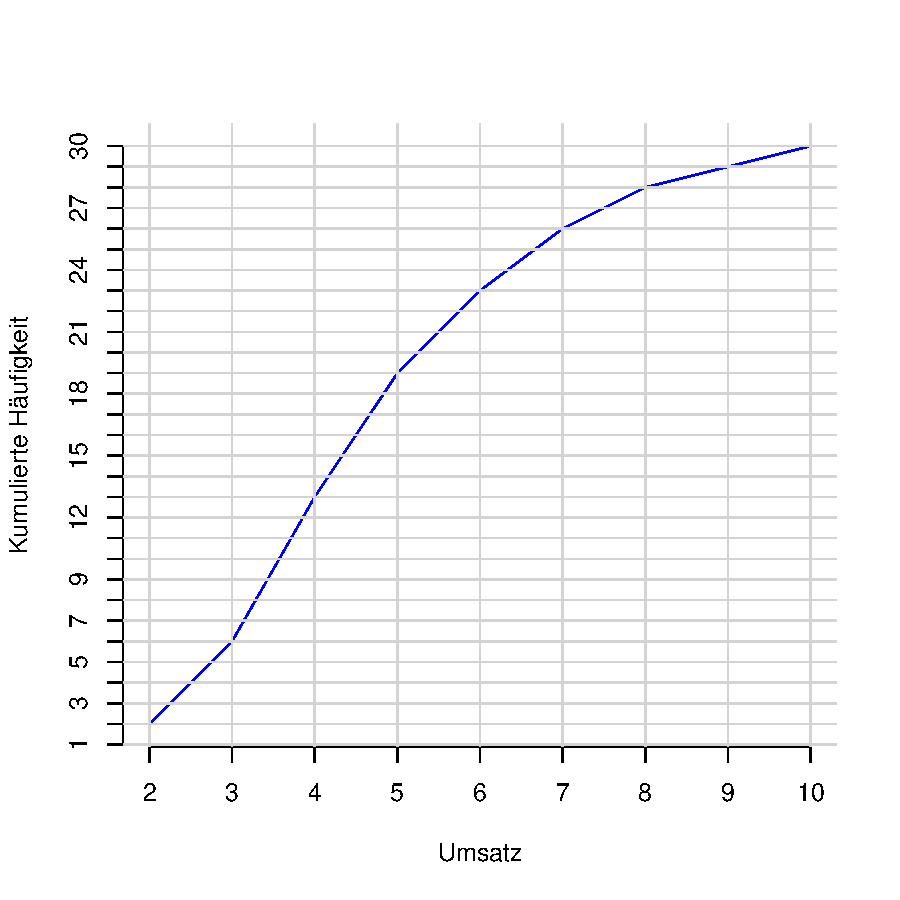
\includegraphics{UEbung2-003}

\subsubsection{c [1,5 ; 3,5), [3,5 ; 5,5), [5,5 ; 7,5),[7,5 ; 9,5), [9,5 ; 11,5)}


\begin{Schunk}
\begin{Sinput}
> #[1,5 ; 3,5), [3,5 ; 5,5), [5,5 ; 7,5),[7,5 ; 9,5), [9,5 ; 11,5) und[1,5 ; 3,5), [3,5 ;6,5),[6,5 ; 10,5) 
> 
> library("graphics")
> income <- c(2, 4, 6, 4, 7, 5, 7, 4, 3, 5,
+             5, 8, 6, 3, 5, 2, 9, 4, 5, 6, 
+             8, 3, 10, 5, 4, 3, 7, 4, 6, 4)
> income.class1 <- income[income >= 1.5 & income < 3.5]
> income.class2 <- income[income >= 3.5 & income < 5.5]
> income.class3 <- income[income >= 5.5 & income < 7.5]
> income.class4 <- income[income >= 7.5 & income < 9.5]
> income.class5 <- income[income >= 9.5 & income < 11.5]
> income.frequency <- c(
+   length(income.class1),
+   length(income.class2),
+   length(income.class3),
+   length(income.class4),
+   length(income.class5)
+ )
> hist(income, breaks = c(1.5, 3.5, 5.5, 7.5, 9.5, 11.5), axes = FALSE, freq = TRUE)
> axis(1, at = c(1.5, 3.5, 5.5, 7.5, 9.5, 11.5), labels = c(1.5, 3.5, 5.5, 7.5, 9.5, 11.5))
> axis(2, at = c(0, income.frequency), labels = c(0, income.frequency))
> 
\end{Sinput}
\end{Schunk}
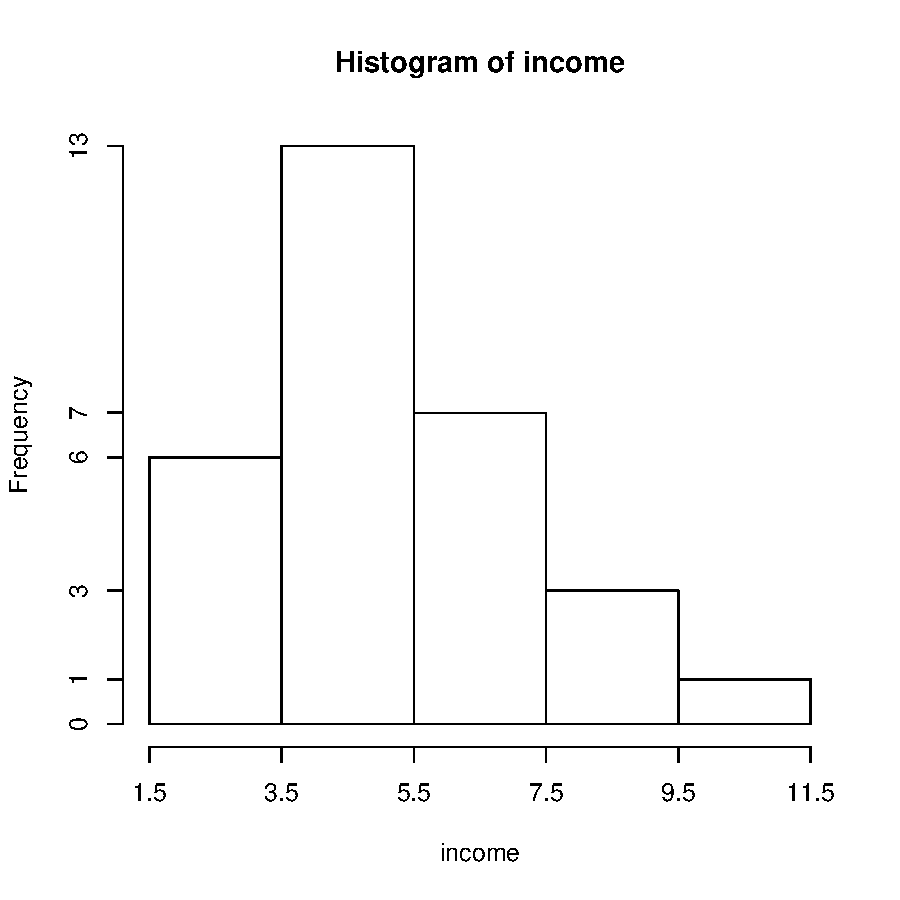
\includegraphics{UEbung2-004}

\subsubsection{c [1,5 ; 3,5), [3,5 ;6,5),[6,5 ; 10,5)}

\begin{Schunk}
\begin{Sinput}
> library("graphics")
> income <- c(2, 4, 6, 4, 7, 5, 7, 4, 3, 5,
+             5, 8, 6, 3, 5, 2, 9, 4, 5, 6, 
+             8, 3, 10, 5, 4, 3, 7, 4, 6, 4)
> income.class6 <- income[income >= 1.5 & income < 3.5]
> income.class7 <- income[income >= 3.5 & income < 6.5]
> income.class8 <- income[income >= 6.5 & income < 10.5]
> income.frequency <- c(
+   length(income.class6),
+   length(income.class7),
+   length(income.class8)
+ )
> breaks <- c(1.5, 3.5, 6.5, 10.5)
> hist(income, breaks = breaks, axes=FALSE, freq = TRUE)
> axis(1, at=breaks, labels=breaks)
> axis(2, at=c(0, income.frequency), labels = c(0, income.frequency))
\end{Sinput}
\end{Schunk}
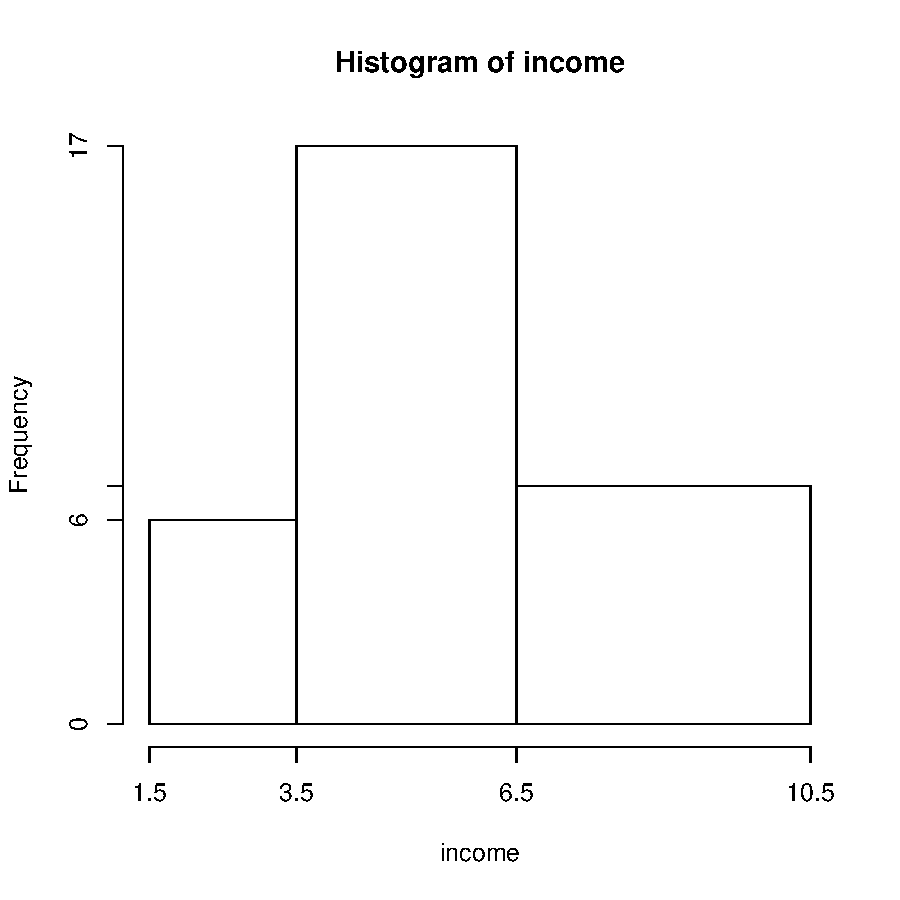
\includegraphics{UEbung2-005}

\subsection{Aufgabe 10}
\subsubsection{a}

\begin{Schunk}
\begin{Sinput}
> children <- c(0, 2, 0, 2, 0, 0, 1, 2, 0, 0, 2, 1, 2, 1, 2, 1, 1, 1, 1, 6, 
+               1 ,2, 0, 2, 0, 0, 1, 0, 0, 1, 0, 0, 1, 0, 0, 1, 1, 0, 2, 1)
> children.table <- table(children);
> children.proptable <- prop.table(children.table)
\end{Sinput}
\end{Schunk}

\begin{Schunk}
\begin{Sinput}
> addmargins(children.table)
\end{Sinput}
\begin{Soutput}
children
  0   1   2   6 Sum 
 16  14   9   1  40 
\end{Soutput}
\begin{Sinput}
> addmargins(children.proptable * 100)
\end{Sinput}
\begin{Soutput}
children
    0     1     2     6   Sum 
 40.0  35.0  22.5   2.5 100.0 
\end{Soutput}
\end{Schunk}

\subsubsection{b}

\begin{Schunk}
\begin{Sinput}
> barplot(children.table, axes = FALSE)
> axis(2, at=0:max(children.table), labels = 0:max(children.table))
\end{Sinput}
\end{Schunk}
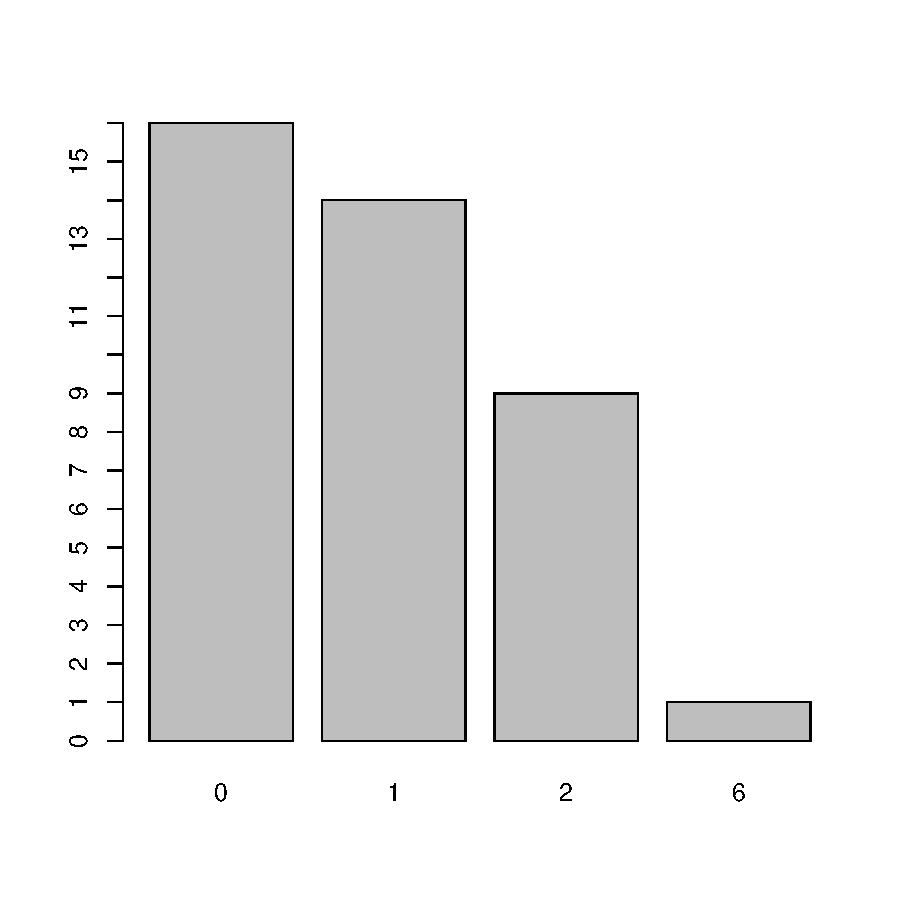
\includegraphics{UEbung2-008}

\begin{Schunk}
\begin{Sinput}
> children.cumsum <- cumsum(children.proptable) * 100
> children.cumsum
\end{Sinput}
\begin{Soutput}
    0     1     2     6 
 40.0  75.0  97.5 100.0 
\end{Soutput}
\begin{Sinput}
> plot(x = children.cumsum, type = "l", col="blue", axes = FALSE, xlab = "", ylab = "")
> axis(1, at = 1:length(children.cumsum), labels = names(children.cumsum))
> axis(2, at = children.cumsum, labels = children.cumsum)
> abline(h = children.cumsum, col="lightgray")
> abline(v = 1:length(children.cumsum), col="lightgray")
\end{Sinput}
\end{Schunk}
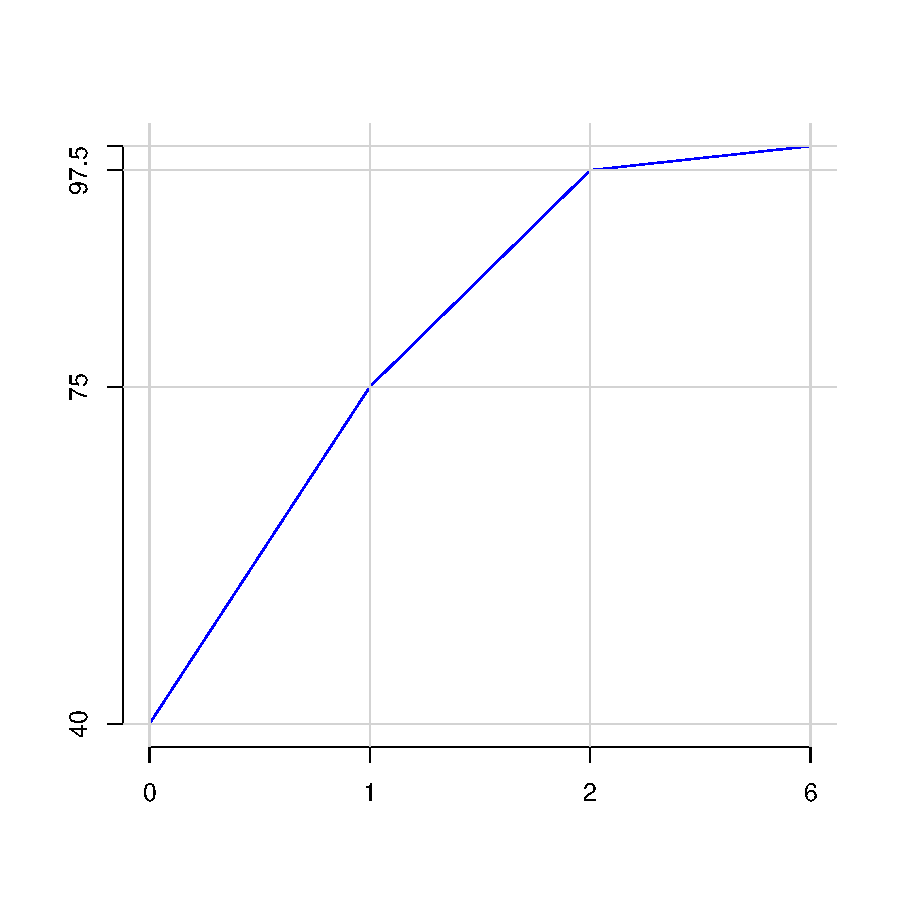
\includegraphics{UEbung2-009}

\subsection{Aufgabe 11}

Therapie A

\begin{Schunk}
\begin{Sinput}
> A.small.all <- 87
> A.small <- 81
> A.small.non <- A.small.all - A.small
> A.big.all <- 263
> A.big <- 192
> A.big.non <- A.big.all - A.big
> A.all <- 350
> A <- 273
> A.non <- A.all - A
> A.prop <- c(A.small / A.all, A.small.non / A.all, A.big / A.all, A.big.non / A.all)
> names(A.prop) <- c("Klein Nierensteine - Erfolg", "Kleine Nierensteine - Kein Erfolg", "Große Nierensteine - Erfolg", "Große Nierensteine - Kein Erfolg")
> A.prop <- round(A.prop * 100, 2)
> A.prop
\end{Sinput}
\begin{Soutput}
      Klein Nierensteine - Erfolg Kleine Nierensteine - Kein Erfolg 
                            23.14                              1.71 
      Große Nierensteine - Erfolg  Große Nierensteine - Kein Erfolg 
                            54.86                             20.29 
\end{Soutput}
\end{Schunk}

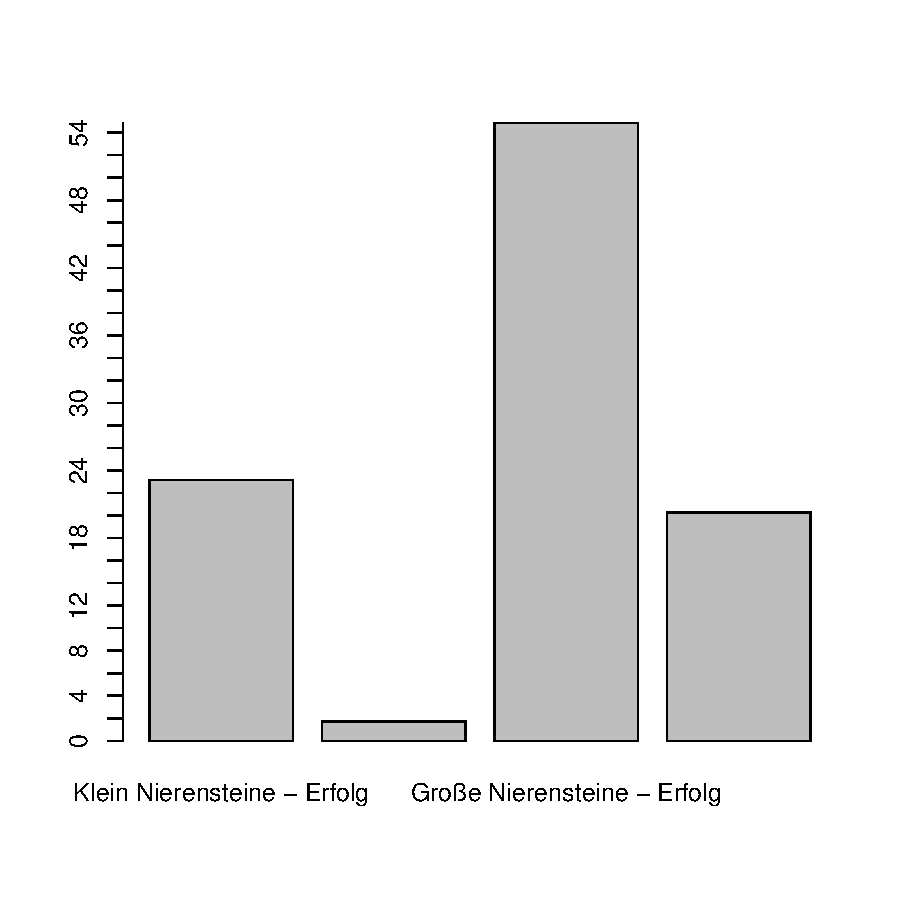
\includegraphics{UEbung2-011}



Therapie B

\begin{Schunk}
\begin{Sinput}
> B.small.all <- 270
> B.small <- 234
> B.small.non <- B.small.all - B.small
> B.big.all <- 80
> B.big <- 55
> B.big.non <- B.big.all - B.big
> B.all <- 350
> B <- 289
> B.non <- B.all - B
> B.prop <- c(B.small / B.all, B.small.non / B.all, B.big / B.all, B.big.non / B.all)
> names(B.prop) <- c("Klein Nierensteine - Erfolg", "Kleine Nierensteine - Kein Erfolg", "Große Nierensteine - Erfolg", "Große Nierensteine - Kein Erfolg")
> B.prop <- round(B.prop * 100, 2)
> B.prop
\end{Sinput}
\begin{Soutput}
      Klein Nierensteine - Erfolg Kleine Nierensteine - Kein Erfolg 
                            66.86                             10.29 
      Große Nierensteine - Erfolg  Große Nierensteine - Kein Erfolg 
                            15.71                              7.14 
\end{Soutput}
\end{Schunk}

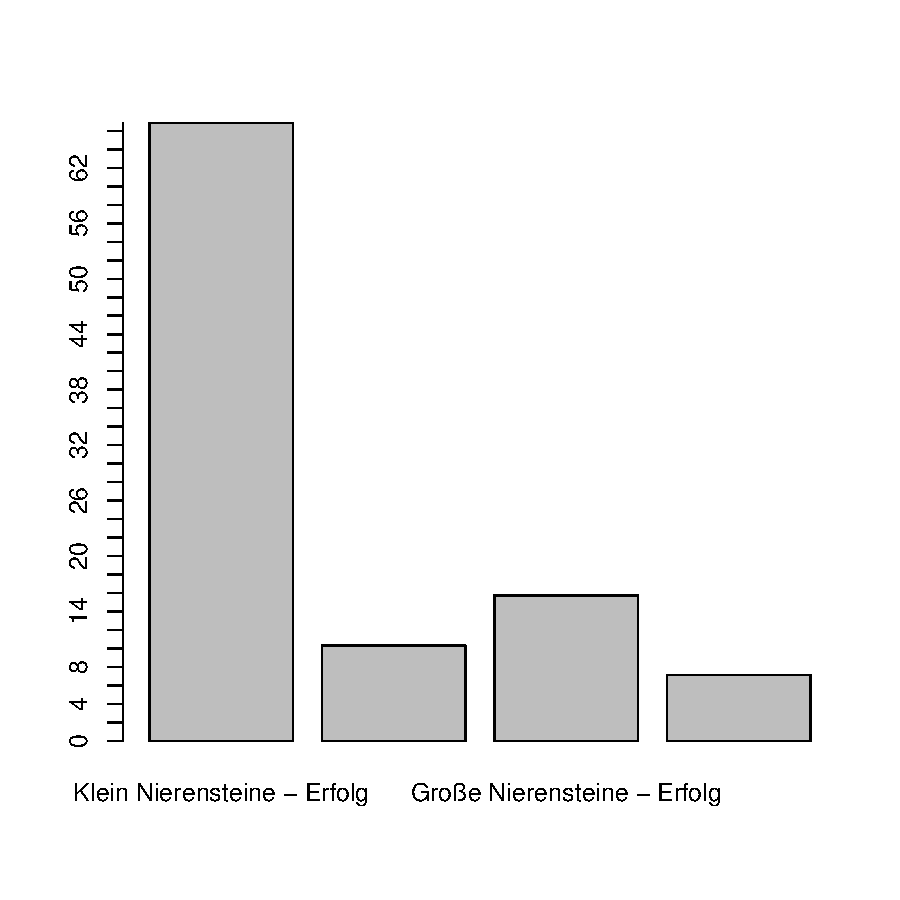
\includegraphics{UEbung2-013}

\subsection{Aufgabe 12}
\subsubsection{a}

\begin{Schunk}
\begin{Sinput}
> classes.calcWidth <- function(begin, end){
+   abs(end - begin)
+ }
> classes.calcMiddle <- function(begin, end){
+   (begin + end) / 2
+ }
> taxpayers <- c(47996, 191492, 124498, 104428, 67988, 31125)
> taxpayers.sum <- sum(taxpayers)
> classes.begin <- c(0, 10, 20, 30, 50)
> classes.end <- c(10, 20, 30, 50, 100)
> classes <- data.frame(
+   Klassen = c("< 10", ">= 10 < 20", ">= 20 < 30", ">= 30 < 50", ">= 50 < 100", " >= 100"),
+   Steuerpflichtige = taxpayers,
+   Breite = c(classes.calcWidth(classes.begin, classes.end), "unbk."),
+   Mitte = c(classes.calcMiddle(classes.begin, classes.end), "unbk."),
+   Häufigkeit = round(taxpayers / taxpayers.sum * 100, 2)
+ )
> classes
\end{Sinput}
\begin{Soutput}
      Klassen Steuerpflichtige Breite Mitte Häufigkeit
1        < 10            47996     10     5       8.46
2  >= 10 < 20           191492     10    15      33.74
3  >= 20 < 30           124498     10    25      21.94
4  >= 30 < 50           104428     20    40      18.40
5 >= 50 < 100            67988     50    75      11.98
6      >= 100            31125  unbk. unbk.       5.48
\end{Soutput}
\end{Schunk}

\subsubsection{b}

Prozentsatz der Fälle mit einer Merkmalsausprägung kleiner 30.000 Euro

\begin{Schunk}
\begin{Sinput}
> cat(sum(classes[c(1,2,3),]$Häufigkeit), "%")
\end{Sinput}
\begin{Soutput}
64.14 %
\end{Soutput}
\end{Schunk}

Prozentsatz der Fälle mit einer Merkmalsausprägung von mindestens 10.000 Euro bis höchstens 50.000 Euro 

\begin{Schunk}
\begin{Sinput}
> cat(sum(classes[c(2,3,4),]$Häufigkeit), "%")
\end{Sinput}
\begin{Soutput}
74.08 %
\end{Soutput}
\end{Schunk}

Prozentsatz der Fälle mit einer Merkmalsausprägung größer 50.000 Euro

\begin{Schunk}
\begin{Sinput}
> cat(sum(classes[c(5,6),]$Häufigkeit), "%")
\end{Sinput}
\begin{Soutput}
17.46 %
\end{Soutput}
\end{Schunk}

\subsection{Aufgabe 13}

\subsubsection{a}

\begin{Schunk}
\begin{Sinput}
> Anzahl <- c(380131, 182838, 87444, 52033, 20235)
> households <- data.frame(
+   Größe = c(1, 2, 3, 4, "5 und mehr", "Summe"),
+   Anzahl = c(Anzahl, sum(Anzahl)),
+   RelativeHäufigkeit = round(c(Anzahl / sum(Anzahl), 1), 3)
+ )
> households
\end{Sinput}
\begin{Soutput}
       Größe Anzahl RelativeHäufigkeit
1          1 380131              0.526
2          2 182838              0.253
3          3  87444              0.121
4          4  52033              0.072
5 5 und mehr  20235              0.028
6      Summe 722681              1.000
\end{Soutput}
\end{Schunk}

\begin{Schunk}
\begin{Sinput}
> barplot(households$RelativeHäufigkeit, names.arg = households$Größe)
\end{Sinput}
\end{Schunk}
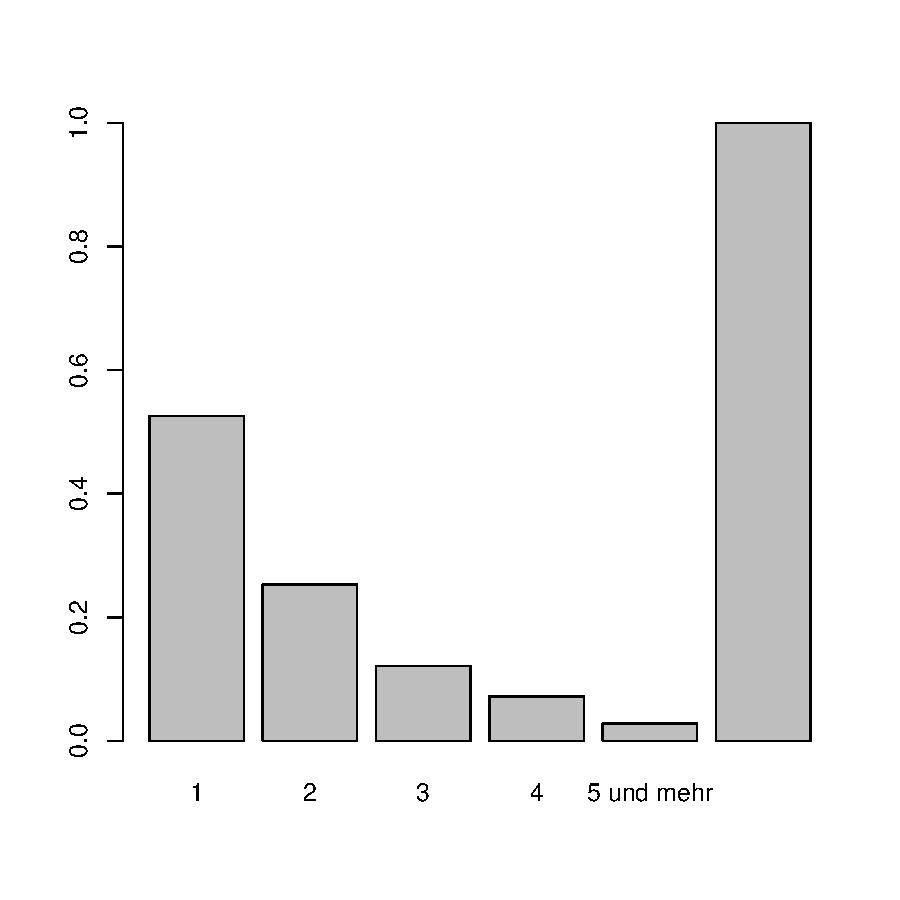
\includegraphics{UEbung2-019}

\subsubsection{b}

„In nahezu 100 Jahren haben sich die Lebensformen stark gewandelt. 
Anfang dieses Jahrhunderts war das Miteinander in der Großfamilie Normalität. 
Fast die Hälfte der Bevölkerung wohnte in Haushalten mit fünf und mehr Personen. 
Ganz anders heute: mehr als die Hälfte der Bevölkerung lebt allein.“

\begin{Schunk}
\begin{Sinput}
> Alone <- households$Anzahl[1] / sum(Anzahl)
> NotAlone <- sum(households$Anzahl[c(-1,-6)])  / sum(Anzahl)
> households.table <- (c(Alone, NotAlone, sum(Alone, NotAlone)))
> names(households.table) <- c("1", "2 und mehr", "Summe")
> households.table
\end{Sinput}
\begin{Soutput}
         1 2 und mehr      Summe 
 0.5260011  0.4739989  1.0000000 
\end{Soutput}
\end{Schunk}
\begin{Schunk}
\begin{Sinput}
> barplot(c(Alone, NotAlone), names.arg = c("1", "2 und mehr"))
\end{Sinput}
\end{Schunk}
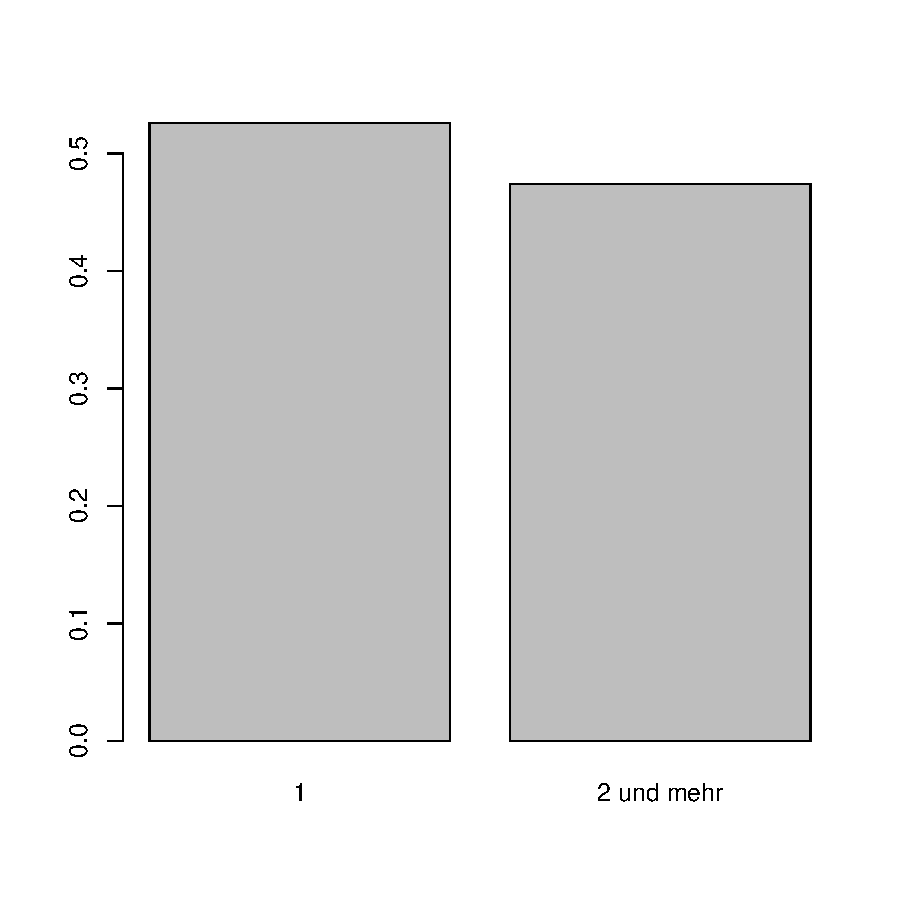
\includegraphics{UEbung2-021}


Anhand des Balkendiagramms kann man erkennen, 
dass tatsächlich mehr als die Hälfte aller Bewohner von München alleine leben.

Um die Aussage der Lebensumstände vor 100 Jahren zu prüfen fehlen die dazugehörigen Daten.

\subsection{Aufgabe 14}

\begin{Schunk}
\begin{Sinput}
> treeHeight <- c(37 , 46 , 42 , 51 , 83 , 79 , 58 , 102 , 130 , 141 , 149 , 152 , 149 , 169 , 171 , 186 , 153 , 190)
> table(treeHeight)
\end{Sinput}
\begin{Soutput}
treeHeight
 37  42  46  51  58  79  83 102 130 141 149 152 153 169 171 186 190 
  1   1   1   1   1   1   1   1   1   1   2   1   1   1   1   1   1 
\end{Soutput}
\end{Schunk}

Klassen:

\begin{table}[htb]
\begin{tabular}{ll}
Klasseneinteilung & Name\\
{[}30,100)        & Klein\\
{[}100, 170)      & Mittel\\
{[}170, Inf)      & Groß
\end{tabular}
\end{table}

\begin{Schunk}
\begin{Sinput}
> Klein <- treeHeight[treeHeight >= 30 & treeHeight < 100]
> Mittel <- treeHeight[treeHeight >= 100 & treeHeight < 170]
> Groß <- treeHeight[treeHeight >= 170]
> trees <- data.frame(
+   Klasse = c(" >= 30 < 100", ">= 100 < 170", ">= 170 < 240"),
+   Klassenbreite = c(70, 70, 70),
+   Klassenmitte = c((30 + 100) / 2, (100 + 170) / 2, (170 + 240) / 2)
+ )
> trees
\end{Sinput}
\begin{Soutput}
        Klasse Klassenbreite Klassenmitte
1  >= 30 < 100            70           65
2 >= 100 < 170            70          135
3 >= 170 < 240            70          205
\end{Soutput}
\end{Schunk}

Klein 

\begin{Schunk}
\begin{Sinput}
> Klein
\end{Sinput}
\begin{Soutput}
[1] 37 46 42 51 83 79 58
\end{Soutput}
\end{Schunk}

Mittel

\begin{Schunk}
\begin{Sinput}
> Mittel
\end{Sinput}
\begin{Soutput}
[1] 102 130 141 149 152 149 169 153
\end{Soutput}
\end{Schunk}

Groß

\begin{Schunk}
\begin{Sinput}
> Groß
\end{Sinput}
\begin{Soutput}
[1] 171 186 190
\end{Soutput}
\end{Schunk}

\begin{Schunk}
\begin{Sinput}
> hist(c(Klein, Mittel, Groß), breaks = c(30, 100, 170, 240), axes = FALSE)
> axis(side = 1, at = c(30, 100, 170, 240), labels = c(30, 100, 170, 240))
> axis(side = 2, at = c(0, length(Klein), length(Mittel), length(Groß)), labels = c(0, length(Klein), length(Mittel), length(Groß)))
\end{Sinput}
\end{Schunk}
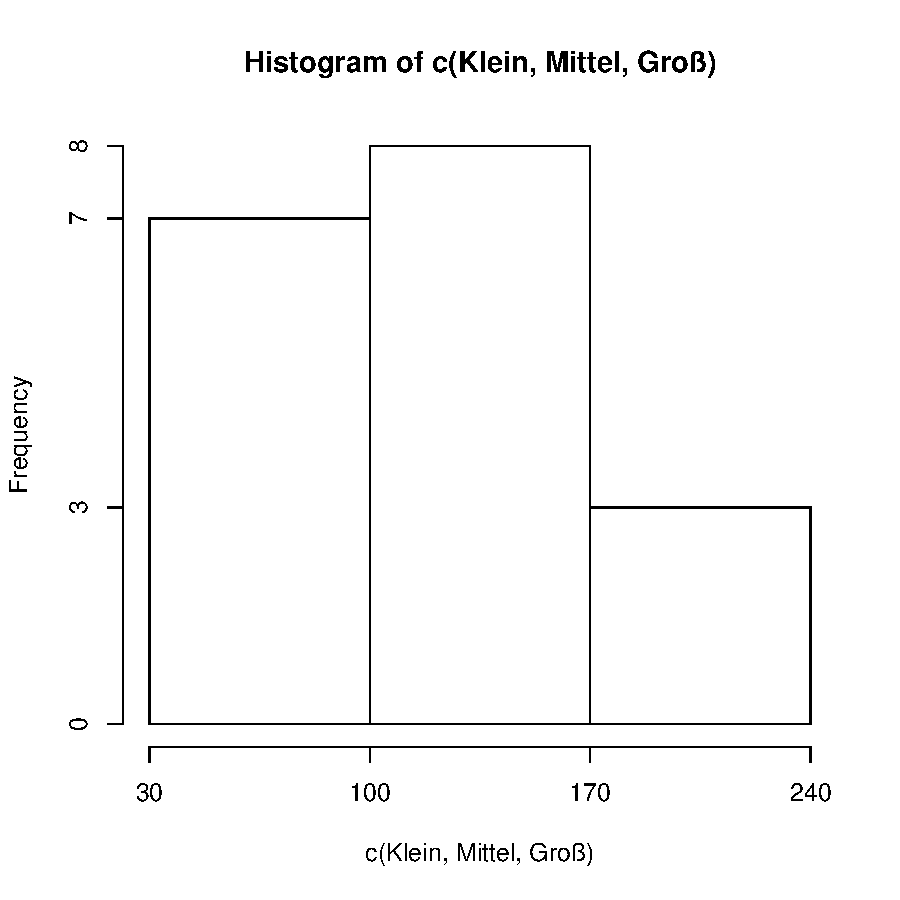
\includegraphics{UEbung2-027}

\subsection{Aufgabe 15}

Merkmal: Anzahl gemeldeter Wohnsitze
Merkmalsausprägungen: 1, 2, 3
50 Personen hatten genau 3 Wohnsitze

\begin{Schunk}
\begin{Sinput}
> places.sum <- 1000
> threePlaces <- 50
> onePlace <- places.sum * 0.8
> twoPlaces <- places.sum - (onePlace + threePlaces)
> places.table <- c(onePlace, twoPlaces, threePlaces)
> names(places.table) <- c("1 Wohnsitz", "2 Wohnsitze", "3 Wohnsitze")
> places.table
\end{Sinput}
\begin{Soutput}
 1 Wohnsitz 2 Wohnsitze 3 Wohnsitze 
        800         150          50 
\end{Soutput}
\begin{Sinput}
> places.tableprop <- prop.table(places.table)
> places.cumsum <- cumsum(places.tableprop)
\end{Sinput}
\end{Schunk}

Tabelle:
\begin{Schunk}
\begin{Sinput}
> places.table
\end{Sinput}
\begin{Soutput}
 1 Wohnsitz 2 Wohnsitze 3 Wohnsitze 
        800         150          50 
\end{Soutput}
\end{Schunk}

Häufigkeitstabelle:
\begin{Schunk}
\begin{Sinput}
> places.tableprop
\end{Sinput}
\begin{Soutput}
 1 Wohnsitz 2 Wohnsitze 3 Wohnsitze 
       0.80        0.15        0.05 
\end{Soutput}
\end{Schunk}

Kummulierte Wahrscheinlichkeiten

\begin{Schunk}
\begin{Sinput}
> places.cumsum
\end{Sinput}
\begin{Soutput}
 1 Wohnsitz 2 Wohnsitze 3 Wohnsitze 
       0.80        0.95        1.00 
\end{Soutput}
\end{Schunk}

\begin{Schunk}
\begin{Sinput}
> plot(x = 0:3, y = c(0, places.cumsum), type="s", axes = FALSE, ylab = "Kumulierte Häufigkeit")
> axis(side = 1, at = c(0:4), labels = c(0:4))
> axis(side = 2, at = seq(from = 0, to = 1, by = 0.1), labels = seq(from = 0, to = 1, by = 0.1))
\end{Sinput}
\end{Schunk}
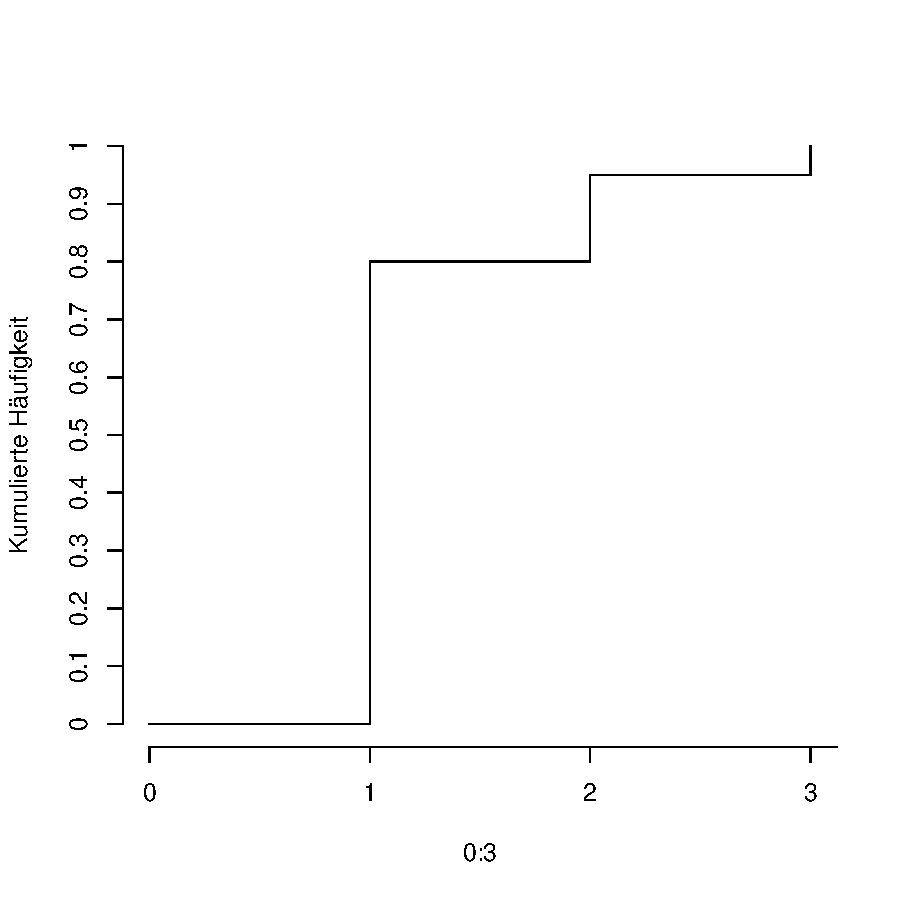
\includegraphics{UEbung2-032}

\subsection{Aufgabe 16}

\begin{Schunk}
\begin{Sinput}
> personPerAge <- c(10, 30, 40, 20)
> personPerAge.data <- personPerAge / 20
\end{Sinput}
\end{Schunk}
\begin{Schunk}
\begin{Sinput}
> barplot(personPerAge.data, axes = FALSE, ylab = "Dichte über absolute Häufigkeit", xlab = "Altersgruppe")
> axis(1, at = 1:4, labels = c(">= 0 < 20", ">= 20 < 40", ">= 40 < 60", ">= 60 < 80"))
> axis(2, at = seq(0, 5, 0.5), labels = seq(0, 5, 0.5))
\end{Sinput}
\end{Schunk}
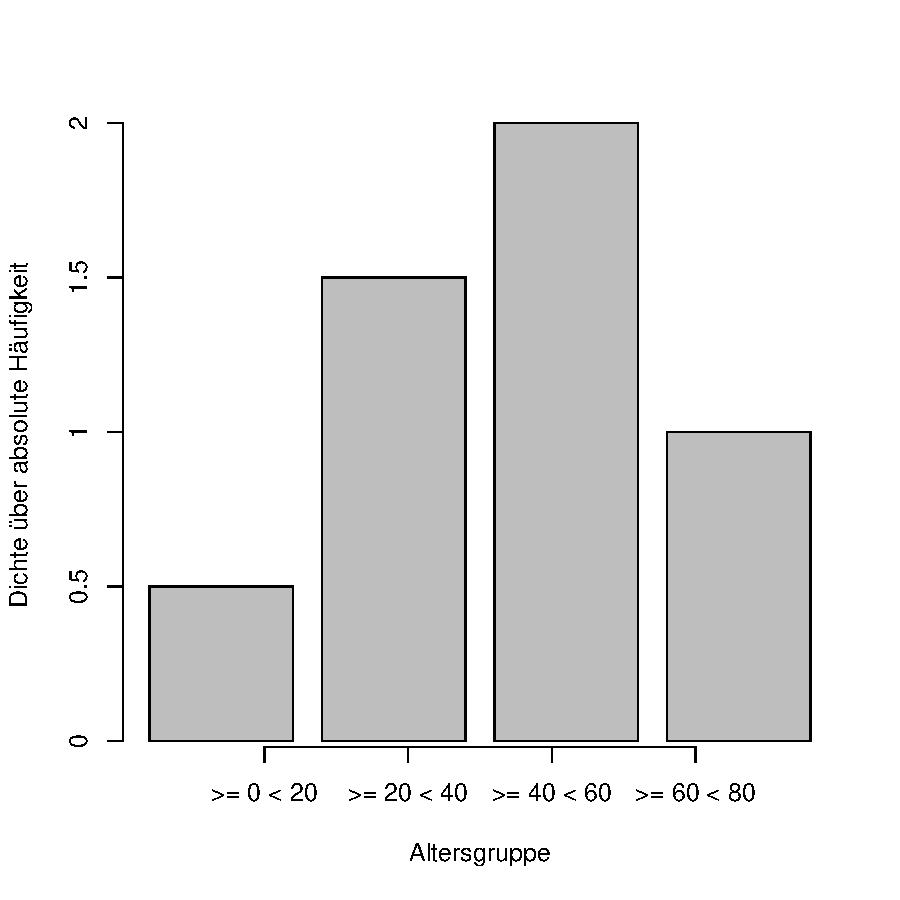
\includegraphics{UEbung2-034}
\begin{Schunk}
\begin{Sinput}
> personPerAge.proptable <- personPerAge / 100
> personPerAge.cumsum <- cumsum(personPerAge.proptable)
> plot(personPerAge.cumsum, type = "l", axes=FALSE, col="blue")
> axis(1, at=1:4, labels = c(">= 0 < 20", ">= 20 < 40", ">= 40 < 60", ">= 60 < 80"))
> axis(2, at = seq(0, 1, 0.1))
> abline(h = personPerAge.cumsum, col="lightgray")
> abline(v = 1:length(personPerAge.cumsum), col="lightgray")
> 
\end{Sinput}
\end{Schunk}
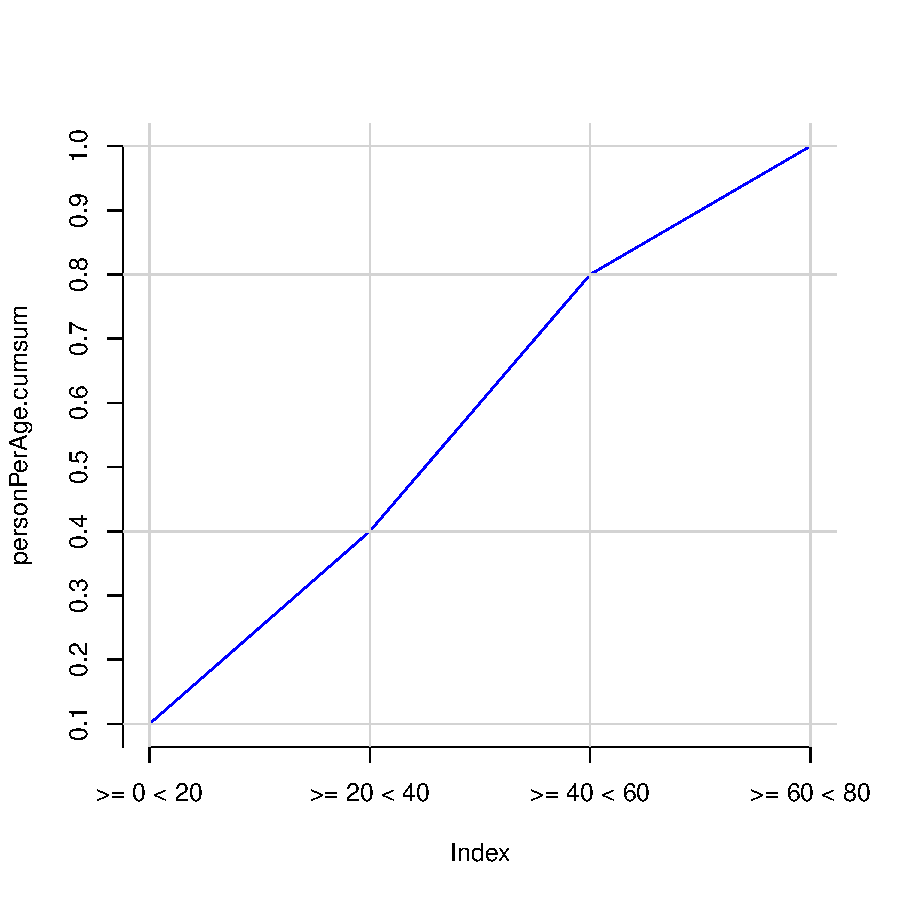
\includegraphics{UEbung2-035}



\end{document}
